\documentclass[a4paper,11pt]{article}
\usepackage[left=2cm, right=2cm, top=2cm, bottom=1.5cm]{geometry}
\usepackage{graphicx}
\usepackage{amssymb}
\usepackage{amsmath}
\usepackage{listings}
\usepackage[utf8]{inputenc}
\usepackage{color} %red, green, blue, yellow, cyan, magenta, black, white
\definecolor{mygreen}{RGB}{28,172,0} % color values Red, Green, Blue
\definecolor{mylilas}{RGB}{170,55,241}

%'codify' text for snippets
\usepackage{xcolor}
\definecolor{codegray}{gray}{0.9}
\newcommand{\code}[1]{	%\colorbox{codegray}  %un-comment for grey box
			{\texttt{#1}}}

\begin{document}
\title{\LARGE{\textbf{ECEN 220 Lab 5\\}}Sampling \& up-scaling}
\author{Niels Clayton \\300437590}
\date{October 6$^{th}$, 2019}
\maketitle
\hrule

\lstset{language=Matlab,%
    %basicstyle=\color{red},
    breaklines=true,%
    morekeywords={matlab2tikz},
    keywordstyle=\color{blue},%
    morekeywords=[2]{1}, keywordstyle=[2]{\color{black}},
    identifierstyle=\color{black},%
    stringstyle=\color{mylilas},
    commentstyle=\color{mygreen},%
    showstringspaces=false,%without this there will be a symbol in the places where there is a space
    %numbers=left,%
    numberstyle={\tiny \color{black}},% size of the numbers
    numbersep=9pt, % this defines how far the numbers are from the text
    emph=[1]{for,end,break},emphstyle=[1]\color{red}, %some words to emphasise
    %emph=[2]{word1,word2}, emphstyle=[2]{style},    
}

\section{Square wave generation \& zero insertion}
Generate a square wave of the following form:\\
\begin{center}
\fbox{\lstinputlisting{square_wave.m}}
\end{center}


\begin{figure}[h]
 \begin{center}
  \fbox{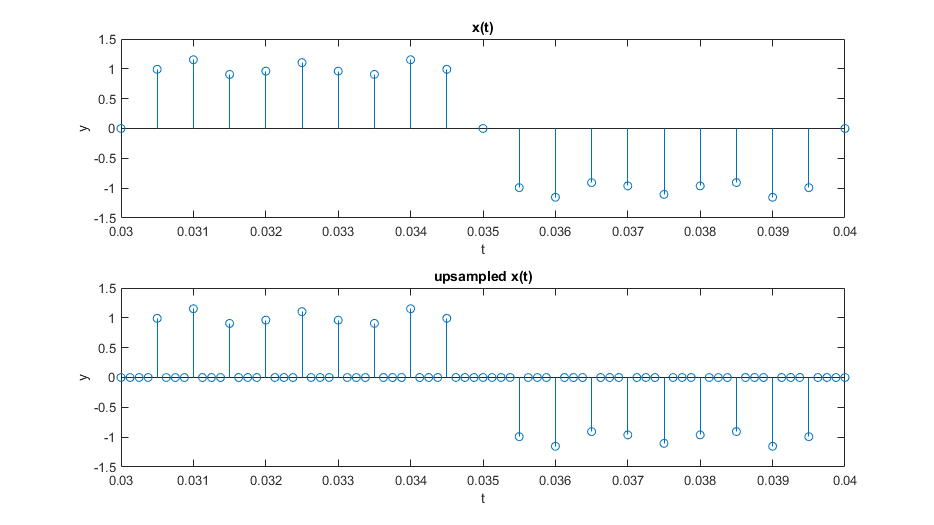
\includegraphics[width = \textwidth]{section1.png}}
  \caption{Original $x[n]$ \& zero inserted $x[n]$}
 \end{center}
\end{figure}

Using the matlab function \code{upsample()} we up-sample the square wave by a factor of 4 by inserting zero values between all the data points.

\pagebreak

\section{Low pass filter generation \& it's frequency response}
Generate a low pass filter of the following form:\\
\begin{center}
\fbox{\lstinputlisting{lowpass.m}}
\end{center}

\begin{figure}[h]
 \begin{center}
  \fbox{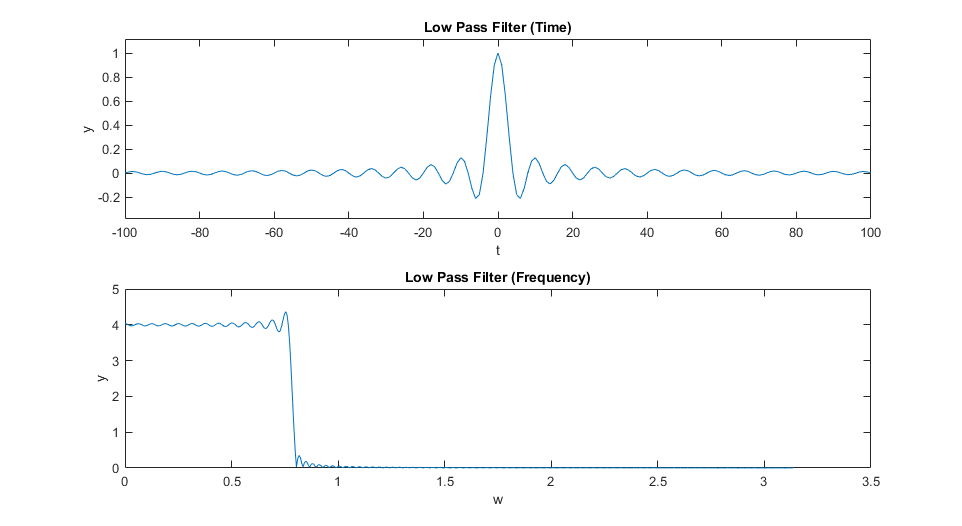
\includegraphics[width = \textwidth]{section2.png}}
  \caption{Low-Pass filter and its frequency response}
 \end{center}
\end{figure}

In figure 2 it can be seen that the low pass filter in time is a $sinc$ function, and a square pulse in frequency. However only the positive half of the square pulse can be observed due to the nature of the Matlab \code{freqz()} function, however we know that it will be symmetrical around the 0 point.\\

After generating this low-pass filter, we will filter the up-sampled square wave with it using the Matlab function \code{filter()} the result of which can be seen below in figure 3, and a phase shifted version can be seen in figure 4 for easier comparisons. 

\pagebreak

\section{Compare the original signal to the up-sampled and filtered signal}

\begin{figure}[h]
 \begin{center}
  \fbox{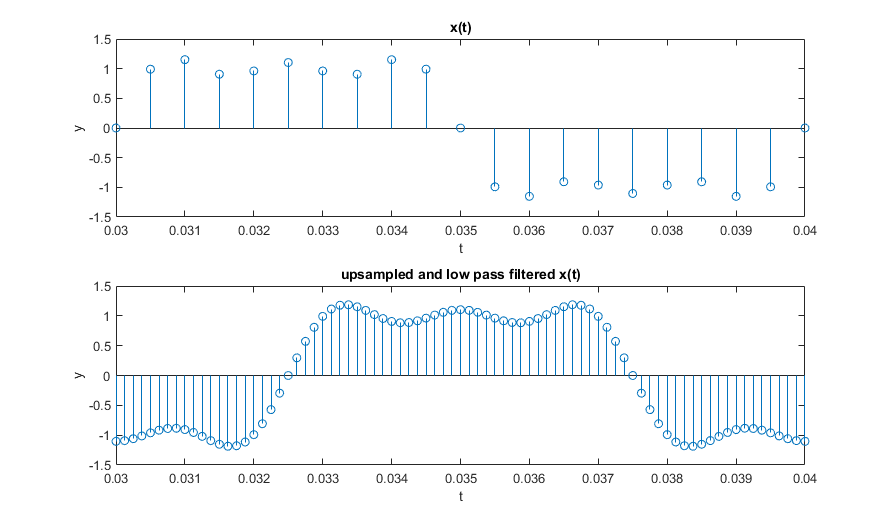
\includegraphics[width = .9\textwidth]{section3.png}}
  \caption{Original signal compared to the up-sampled signal}
  \vspace{-30pt}
 \end{center}
\end{figure}

\section{Phase shift the up-sampled and filtered signal}

\begin{figure}[h]
 \begin{center}
  \fbox{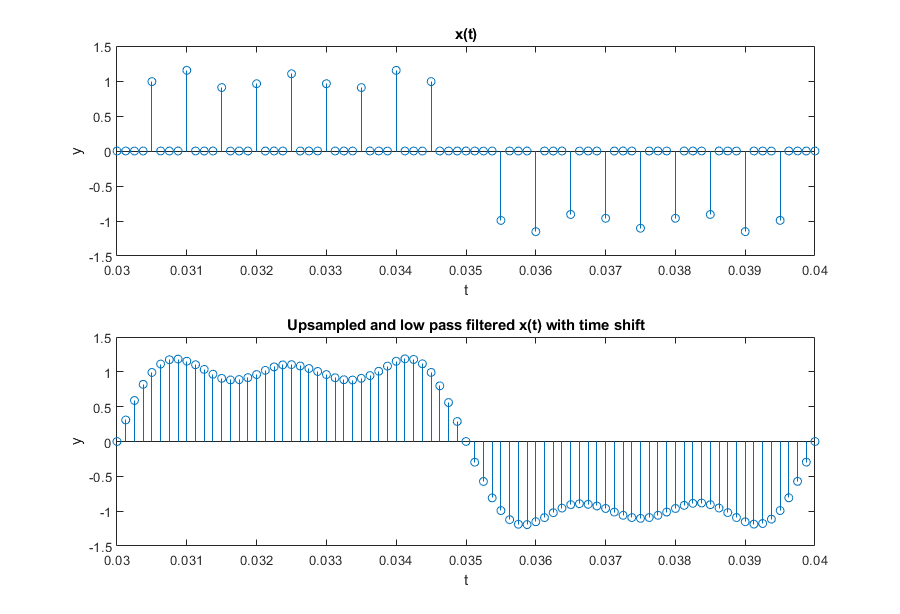
\includegraphics[width = .9\textwidth]{section4.png}}
  \caption{Up-sampled signal phase shifted for easier comparison}
    \vspace{-80pt}
 \end{center}
\end{figure}
\vspace{60pt}

It can be seen that the up-sampled signal is very close if not identical to the information held within the original signal. 

\pagebreak

\lstinputlisting{lab_5.m}

\end{document}







